
%%%%%%%%%%%%%%%%%%%%%%% file typeinst.tex %%%%%%%%%%%%%%%%%%%%%%%%%
%
% This is the LaTeX source for the TDPTemplate using
% the LaTeX document class 'llncs.cls' Springer LNAI format
% used in the RoboCup Symposium submissions.
% http://www.springer.com/computer/lncs?SGWID=0-164-6-793341-0
%
% It may be used as a template for your own TDP - copy it
% to a new file with a new name and use it as the basis
% for your Team Description Paper
%
% NB: the document class 'llncs' has its own and detailed documentation, see
% ftp://ftp.springer.de/data/pubftp/pub/tex/latex/llncs/latex2e/llncsdoc.pdf
%
%%%%%%%%%%%%%%%%%%%%%%%%%%%%%%%%%%%%%%%%%%%%%%%%%%%%%%%%%%%%%%%%%%%

\documentclass[runningheads,a4paper]{llncs}
\usepackage{amssymb}
\setcounter{tocdepth}{3}
\usepackage{graphicx}
\usepackage{amssymb}
\usepackage[utf8]{inputenc}
\usepackage{url}
\usepackage{float}
\usepackage{amsmath}
\usepackage{graphicx}
\usepackage{wrapfig}
\usepackage{tabto}
\usepackage{lipsum}
\usepackage[table,xcdraw]{xcolor}
\usepackage{hyperref}

\begin{document}


\newif\ifdraft
\draftfalse

\title{Walking Machine @Home \newline \: 2018 Team Description Paper}

\author{Jeffrey Cousineau and Philippe La Madeleine}
\institute{École de Technologie Supérieure \\ 1100 rue Notre-Dame Ouest, Montreal, QC, Canada H3C 1K3 \\
\texttt{http://walkingmachine.ca,} \texttt{walking@ens.etsmtl.ca,} \texttt{https://github.com/WalkingMachine}}
\maketitle


%%%%%%%%%%%%%%%%%%%%%%%%%%%%%%%%%%%%%%%%%%%%%%%%%%%%%%%%%%%%%%%%%%%%%%%%%%%%%%%%%%%%

\begin{abstract}

This paper gives details about the RoboCup@Home league team Walking Machine, from ETS University in Montreal, Canada for the next competition in his hometown, Montreal, in July 2018. The robot from Walking Machine, named SARA for "Système d’Assistance Robotique Autonome" (in English, Automated Robotic Assistance System), is a robot entirely built by the scientific club from ETS, mainly composed of undergraduates students. The robot is used for social interaction with humans, navigation and object manipulation. This document shows the electrical, mechanical and software properties and functionalities of SARA. It specifically emphasizes on human following, object and people recognition as well as navigation, manipulation and human-robot interaction.

\end{abstract}

%%%%%%%%%%%%%%%%%%%%%%%%%%%%%%%%%%%%%%%%%%%%%%%%%%%%%%%%%%%%%%%%%%%%%%%%%%%%%%%%%%%%

\section{Introduction}
\tab Walking Machine’s team is a young team from Montreal, Quebec, in Canada, composed of engineering student in the field of mechanical, electrical and software engineering. We have been working on our robot for the last year in prevision of the Robocup at Home competition. As this would be our third participation, we learned a lot on our second attempt last year and have made various modifications to get better results, mostly on the software side. In the past, the team went in many competitions like the Eurobot, but made the leap for the RoboCup@Home competition to get a bigger challenge. \\

SARA, our creation, was designed for polyvalent human-robot interaction as well as efficient navigation and object manipulation. Our robot is mounted on four mecanum wheels powered by Roboteq drives, has one arm mimicking a normal human arm, and sensors for communication and navigation. Our team has developed knowledge in object and people detection/recognition, as well as navigation using a laser scanner, odometry on the wheels and a Asus Xtion camera. All of these parts are interfaced through ROS (Robot Operating System). \\

\section{Electrical and mechanical design of SARA}
\subsection{Electrical}


\subsection{Mechanical}


\section{Software}

\subsection{High-level task planning}
\tab For our task planning, we use a state machine software developed by team Vigir, one of the participant of the Darpa Robotics Challenge. This software is named \href{http://philserver.bplaced.net/fbe/index.php}{FlexBe}, for Flexible Behavior, is a block based interface for making state machines.\\

But we do not simply use FlexBe as is. We still need write our own blocks for it using its python API. To simplify our work, we started by splitting all of the Robocup@home scenarios into basic actions. We then identified all of these basic actions our platform could accomplish and we confined them in blocks named States, e.g. MoveArm, MoveHead etc. These blocks can then be assembled together to form a higher level of blocs we named Actions e.g. Pick, LookAt etc. Those Actions can then again be assembled into what we call ActionWrappers. The role of ActionWrapper is to allow interfacing our Actions with our natural language processing software(see natural language processing below). They receive the segmented text and translate it to computer understandable parameters using our Wonderland (see environment reasoning below) knowledge base and other sources of informations. This recursive structure allow us allow us to quickly develop our robot’s behaviours.

\subsection{Natural language processing}
\tab To analyse the detected speech, we rely on a software develop by the  \href{http://sag.art.uniroma2.it/}{Semantic analytic group from the University of Roma} and the \href{http://labrococo.dis.uniroma1.it/}{Laboratory of Cognitive Cooperating Robots} at Sapienza University of Rome. This speech analyzer, named \href{http://sag.art.uniroma2.it/lu4r.html}{LU4R} for “Language Understanding For Robots”, is composed of a server developed in Java which take as an input the detected sentence and the semantic environment surrounding the robot.\\

This server communicate through a REST service which give him the possibility to be compliant with all kind of platform. All you have to do is to launch the server locally which is compiled through a .jar file. Again, this give the opportunity to use this software on every platform, whether you’re on Windows, Linux or Mac. \\

This software gives you the possibility to get different output representation. We choose the \href{https://github.com/amrisi/amr-guidelines/blob/master/amr.md}{amr representation} since it was the easiest one to understand and to implement.\\

We decided to build our own ROS wrapper, \href{https://github.com/WalkingMachine/lu4r_ros}{lu4r\_ros}  to better interface it with our task planning approach. We first translate the response given by LU4R into simple format we call ActionForms. The ActionForms contains an action followed by all of its possible parameters as identified in the \href{https://framenet2.icsi.berkeley.edu/fnReports/data/luIndex.xml}{FrameNet Index of Lexical Units}
The ActionWrappers are then fed into a FIFO based priority manager and finally send to our task planner.\\

What is also interesting about LU4R, it’s that it will use the semantic mapping in it’s analysing process. All you have to do is to provide the correct pose for every object in the robot’s environment. You can also precise various synonym for every object to get a better understanding of inputted sentence.\\

\ifdraft
\begin{figure}
  \centering
  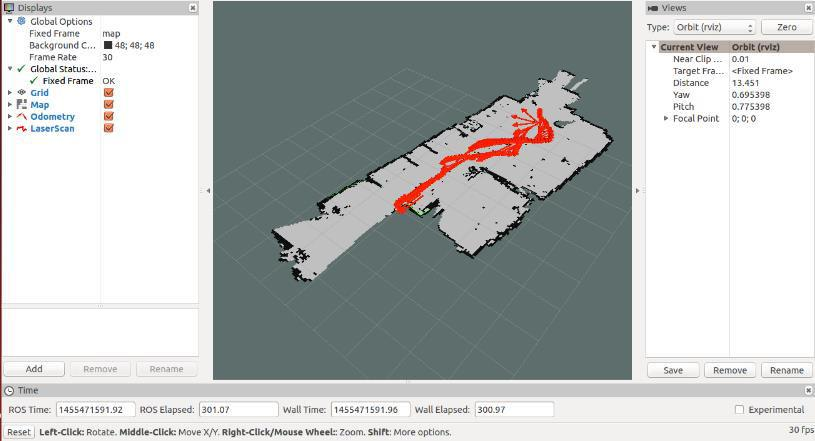
\includegraphics[width=150pt]{images/map.jpg}
  \caption{Mapping}
\end{figure}
\fi



\subsection{Object recognition}
\tab As a beginning team, we are still exploring various solution around the object recognition problem. Our first plan was to use the object recognition kitchen package from Willow Garage. But after using it in competition, we realised that the performance and the easiness to use wasn’t what the approach we were looking for. As an alternative, we start using the YOLO (You Only Look Once) ros package (link). \\

YOLO is a real-time object detection. It does not only detect various object but it also predict the bounding boxes of the detected object. It use a single neural network which is applied to the image. Multiple regions are then created and are used to predict the bounding boxes. Each bounding boxes also contain are predicted probability which are used to filter the predicted objects. The advantage of this system is that it can detect multiple objects in a real-time scenario.\\
 
We use the ROS package to make our job easier since this gave us the possibility to directly get the recognized objects output into a ROS topic. We can also get the bounding box for each detected object. First step we had to do was to transform those 2D bounding boxes in 3D to get a specific pose according to our robot. \\

[Image expliquant 2d bounding boxe -> 3D pose]\\

For the moment, we created the package \href{https://github.com/WalkingMachine/wm_frame_to_box}{wm\_frame\_to\_box} to approximate the object pose by the depth point of the center of the bounding box. Even though it can have flaws, this technique has also proven to be largely sufficient for most of our applications and most importantly, it uses way less processing power than the full 3D pattern matching we used before. This allow us to do real time object positioning, a capability we are proud of.\\

[Image expliquant la prochaine technique, bounding box -> pointcloud seg -> haf grasp] \\

Afterward, to get better results and a better pose, we plan to substract the point cloud according to the bounding boxes. We will then use it with the pointcloud segmentation from the \href{http://pointclouds.org}{PCL library} to extract the specific object and send it to a grasp identification package like \href{http://http://wiki.ros.org/haf_grasping}{haf\_grasping}. This technique, compare to what we are actually using would give us the possibility to grab a much wider variety of object.\\

For the moment, we are using the COCO model but, we are looking forward to train our own dataset, just like we would do in competition. As an undergrad team, this is new for us but we have all the tools we need to overcome this. \\

\ifdraft
\begin{figure}
  \centering
  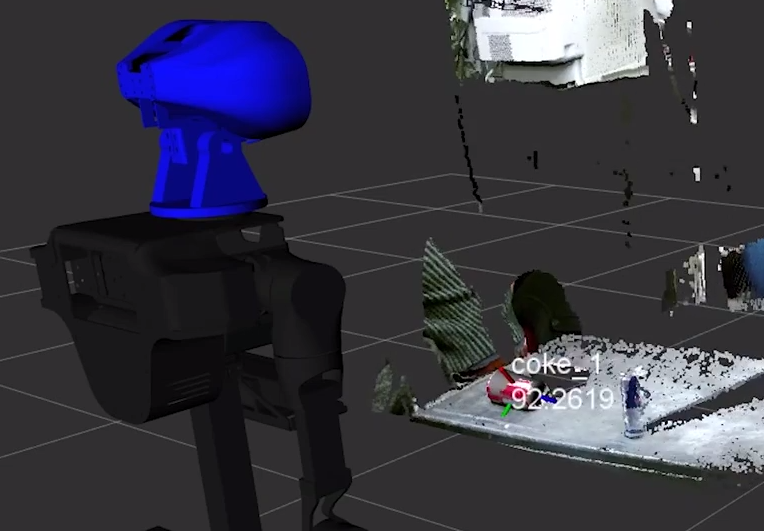
\includegraphics[width=150pt]{images/objectreco.png}
  \caption{Object recognition}
\end{figure}
\fi

\newpage
\subsection{Navigation}
\tab  

\subsection{Environmental reasoning}
\tab In addition of last year navigation stack, this year we are using the pointcloud-to-lasercan package as a lighter solution for 3D navigation. We still use octomap as part of the collision avoidance system for the moveit arm planning.\\



\section{Conclusions and future work}
\tab As you can see, since last year, we made large progress, starting with the improvement of our object detection module. Also, the implementation of a semantic representation of the environment is a big step for us since it helps our robot to have a better understanding of his surrounding. Finally, the various mechanicals modifications will help for a better navigation and a better management of our robot. So SARA is now a completely autonomous system able of interaction with the human as well as navigation in her environment. Using his multiple sensors, like laser sensor, depth camera, IMU and odometry our robot can analyse his environment, recognize people and objects and navigate through obstacles. It can then interact with objects and people using his voice recognition and voice synthesis abilities to keep track of his state. All of the requirements for the Robocup@home are met by SARA and it's a fast-evolving robot considering the team is really young and composed of undergraduates in various engineering programs. As future works, we will add a second arm to give us the possibility for two-hands manipulation. Also, we'll add a vertical translation to our body to give our robot a larger range for objects manipulation.\\

\section*{Robot SARA Hardware Description}
% TODO Change picture and description
Specifications for robot SARA are as follows:

\begin{table}

\label{my-label}

\begin{tabular}{l|p{90mm}}
\hline
\rowcolor[HTML]{FFFFFF} 
\multicolumn{2}{c}{\cellcolor[HTML]{FFFFFF}\textbf{SARA}}                                                      \\ \hline
\rowcolor[HTML]{EAEFF6} 
\textbf{Base}               & Custom base with fully holonomic platform                                        \\
\rowcolor[HTML]{FFFFFF} 
\textbf{Right arm}          & 7 DoF custom arm made of Kinova motors                                           \\
\rowcolor[HTML]{EAEFF6} 
\textbf{Neck}               & Tilt and pan unit using two Dynamixel MX-64R servo actuator                      \\
\rowcolor[HTML]{FFFFFF} 
\textbf{Head}               & Custom head made of RGB neopixels leds and Asus Xtion Pro                        \\
\rowcolor[HTML]{EAEFF6} 
\textbf{Gripper}            & Robotiq 2 fingers 140mm                                                           \\
\rowcolor[HTML]{FFFFFF}
\textbf{Dimensions}         & \begin{tabular}[c]{@{}l@{}}Base : 0,61m. X 0,77m.\\ Height : 1,68m.\end{tabular} \\
\rowcolor[HTML]{EAEFF6} 
\textbf{Weight}             & $\sim$60kg                                                                      \\
\rowcolor[HTML]{FFFFFF} 
\textbf{Additional sensors} & Hokuyo UTM-30LX on base                                                          \\
\rowcolor[HTML]{EAEFF6} 
\textbf{Microphone}         & Rode microphone											                         \\
\rowcolor[HTML]{FFFFFF} 
\textbf{Batteries}          & 2x 20V Dewalt drill battery 5aH                                                 \\
\rowcolor[HTML]{EAEFF6} 
\textbf{Computer}           & 1x Lenovo p50 with 32GB RAM and nVidia Quadro M2000 4GB, 1x Raspberry Pi 3       \\ \hline
\end{tabular}
\caption{Robot's hardware description}
\end{table}
\begin{wrapfigure}[10]{r}{0.25\textwidth}
	\centering
	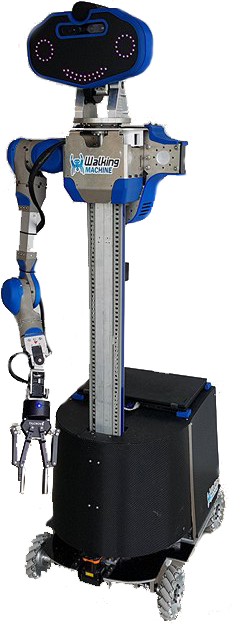
\includegraphics[width=0.30\textwidth]{images/sara_2.png}
	\caption{Robot SARA}
\end{wrapfigure}
\section*{Robot's Software Description}

For our robot we are using the following software:

\begin{itemize}
	\item Platform: Robotic Operating System (ROS) Kinetic on Ubuntu 16.04
	\item Navigation, localization and mapping: \href{http://wiki.ros.org/gmapping}{Gmapping}, \href{http://wiki.ros.org/amcl}{AMCL}, \href{http://wiki.ros.org/pointcloud_to_laserscan}{pointcloud\_to\_laserscan}
	\item Face recognition: \href{http://wiki.ros.org/people}{People}
	\item Speech recognition: \href{https://github.com/WalkingMachine/lab_ros_speech_to_text}{Google Speech API}
	\item Speech comprehension: \href{http://sag.art.uniroma2.it/lu4r.html}{LU4R}, \href{https://github.com/WalkingMachine/lu4r_ros}{lu4r\_ros}
	\item Speech generation: \href{https://doc.ubuntu-fr.org/svoxpico}{Svoxpico}
	\item Object recognition: \href{https://github.com/WalkingMachine/wm_darknet}{Darknet with YOLO v2 }
	\item Arm control: \href{http://wiki.ros.org/moveit}{MoveIt} and \href{https://github.com/Kinovarobotics/kinova-ros}{Kinova API}
	\item Task executor: \href{http://wiki.ros.org/flexbe}{Flexbe} 
	\item World reprensentation: \href{http://github.com/walkingmachine/wonderland}{Wonderland}
\end{itemize}
	

\section*{Team members}
Jeffrey Cousineau, Philippe La Madeleine, Maxime St-Pierre, Jimmy Poirier, Philippe La Madelaine, Samuel Otis, Redouane Laref, Louis-Charle Labarre, Lucas Maurice, Léonore Jean-François, Nicolas Nadeau 

\nocite{*}
\bibliographystyle{plain}
\bibliography{references}


\end{document} 
